\documentclass[12pt]{article}

% Paquetes necesarios
\usepackage{amsthm}
\usepackage{amsmath}
\usepackage{amssymb}
\usepackage{geometry}
\usepackage{graphicx}
\usepackage{hyperref}
\usepackage{fancyhdr}
\usepackage{enumitem}
\usepackage{tikz}
\usepackage{tikz-3dplot}
\usepackage{pgfplots}
\pgfplotsset{compat=1.18}
\usetikzlibrary{angles,patterns,calc,intersections,decorations.markings,arrows.meta,3d}

% Configuración de márgenes
\geometry{a4paper, margin=1in}

% Aumentamos la altura del encabezado
\setlength{\headheight}{15pt}

% Definición de entornos
\newtheorem{theorem}{Teorema}[section]
\newtheorem{definition}[theorem]{Definición}
\newtheorem{example}[theorem]{Ejemplo}
\newtheorem{proposition}[theorem]{Proposición}
\newtheorem{corollary}[theorem]{Corolario}

% Encabezado
\pagestyle{fancy}
\fancyhead[L]{Geometría Vectorial}
\fancyhead[R]{\thepage}

\title{\textbf{Geometría Vectorial} \\ \large Cheatsheet Completo y Extenso}
\author{Jaime Sebastian Chavarria Fuertes}
\date{\today}

\begin{document}

\maketitle
\tableofcontents
\newpage

\section{Fundamentos de Vectores}

\subsection{Definiciones Básicas}

\begin{definition}
Un \textbf{vector} es un objeto matemático que tiene magnitud (longitud) y dirección. Se representa como $\vec{v}$ o $\mathbf{v}$.
\end{definition}

\textbf{Notación}:
\begin{itemize}
  \item Vector en 2D: $\vec{v} = (v_x, v_y)$ o $\vec{v} = v_x\vec{i} + v_y\vec{j}$
  \item Vector en 3D: $\vec{v} = (v_x, v_y, v_z)$ o $\vec{v} = v_x\vec{i} + v_y\vec{j} + v_z\vec{k}$
  \item Vector en n-D: $\vec{v} = (v_1, v_2, \ldots, v_n)$
\end{itemize}

\subsection{Operaciones Vectoriales Básicas}

\subsubsection{Suma de vectores}

\[
\boxed{
\vec{u} + \vec{v} = (u_1 + v_1, u_2 + v_2, u_3 + v_3)
}
\]

\textbf{Propiedades}:
\begin{itemize}
  \item Conmutativa: $\vec{u} + \vec{v} = \vec{v} + \vec{u}$
  \item Asociativa: $(\vec{u} + \vec{v}) + \vec{w} = \vec{u} + (\vec{v} + \vec{w})$
  \item Elemento neutro: $\vec{v} + \vec{0} = \vec{v}$
  \item Elemento inverso: $\vec{v} + (-\vec{v}) = \vec{0}$
\end{itemize}

\subsubsection{Resta de vectores}

\[
\boxed{
\vec{u} - \vec{v} = (u_1 - v_1, u_2 - v_2, u_3 - v_3)
}
\]

\subsubsection{Multiplicación por escalar}

\[
\boxed{
k\vec{v} = (kv_1, kv_2, kv_3)
}
\]

\textbf{Propiedades}:
\begin{itemize}
  \item Asociativa: $(kl)\vec{v} = k(l\vec{v})$
  \item Distributiva respecto a suma de vectores: $k(\vec{u} + \vec{v}) = k\vec{u} + k\vec{v}$
  \item Distributiva respecto a suma de escalares: $(k + l)\vec{v} = k\vec{v} + l\vec{v}$
  \item Elemento neutro: $1\vec{v} = \vec{v}$
\end{itemize}

\subsection{Magnitud (Norma) de un Vector}

\subsubsection{En 2D}

\[
\boxed{
|\vec{v}| = \|\vec{v}\| = \sqrt{v_x^2 + v_y^2}
}
\]

\subsubsection{En 3D}

\[
\boxed{
|\vec{v}| = \|\vec{v}\| = \sqrt{v_x^2 + v_y^2 + v_z^2}
}
\]

\subsubsection{En n-D}

\[
\boxed{
|\vec{v}| = \sqrt{\sum_{i=1}^{n} v_i^2}
}
\]

\subsection{Vector Unitario}

Un vector unitario tiene magnitud 1.

\[
\boxed{
\hat{v} = \frac{\vec{v}}{|\vec{v}|}
}
\]

\textbf{Vectores unitarios estándar}:
\begin{itemize}
  \item En 2D: $\vec{i} = (1, 0)$, $\vec{j} = (0, 1)$
  \item En 3D: $\vec{i} = (1, 0, 0)$, $\vec{j} = (0, 1, 0)$, $\vec{k} = (0, 0, 1)$
\end{itemize}

\subsection{Dirección de un Vector}

En 2D, el ángulo que forma con el eje $x$ positivo:

\[
\boxed{
\theta = \arctan\frac{v_y}{v_x}
}
\]

En 3D, los ángulos directores $\alpha, \beta, \gamma$ con los ejes $x, y, z$:

\[
\boxed{
\cos\alpha = \frac{v_x}{|\vec{v}|} \quad , \quad \cos\beta = \frac{v_y}{|\vec{v}|} \quad , \quad \cos\gamma = \frac{v_z}{|\vec{v}|}
}
\]

Y se cumple: $\cos^2\alpha + \cos^2\beta + \cos^2\gamma = 1$

\subsection{Ilustración: Suma de vectores}

\begin{center}
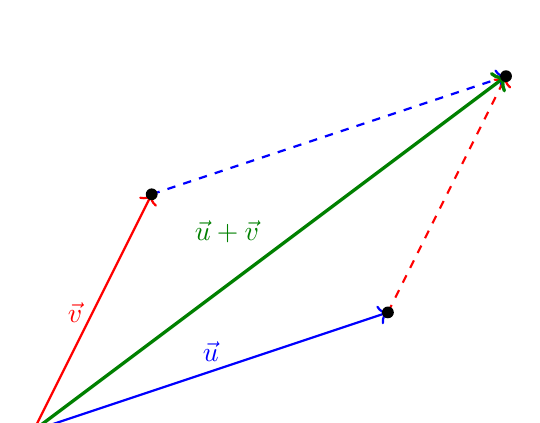
\begin{tikzpicture}[scale=1.5]
  % Vectores
  \draw[->, thick, blue] (0,0) -- (3,1) node[midway, above] {$\vec{u}$};
  \draw[->, thick, red] (0,0) -- (1,2) node[midway, left] {$\vec{v}$};
  
  % Método del paralelogramo
  \draw[->, thick, blue, dashed] (1,2) -- (4,3);
  \draw[->, thick, red, dashed] (3,1) -- (4,3);
  
  % Vector resultante
  \draw[->, very thick, green!50!black] (0,0) -- (4,3) node[midway, above left] {$\vec{u} + \vec{v}$};
  
  % Puntos
  \fill (0,0) circle (0.05);
  \fill (3,1) circle (0.05);
  \fill (1,2) circle (0.05);
  \fill (4,3) circle (0.05);
\end{tikzpicture}
\end{center}

\section{Producto Punto (Escalar)}

\subsection{Definición}

\[
\boxed{
\vec{u} \cdot \vec{v} = u_1v_1 + u_2v_2 + u_3v_3 = |\vec{u}||\vec{v}|\cos\theta
}
\]

donde $\theta$ es el ángulo entre los vectores.

\subsection{Propiedades del Producto Punto}

\begin{enumerate}
  \item \textbf{Conmutativa}: $\vec{u} \cdot \vec{v} = \vec{v} \cdot \vec{u}$
  
  \item \textbf{Distributiva}: $\vec{u} \cdot (\vec{v} + \vec{w}) = \vec{u} \cdot \vec{v} + \vec{u} \cdot \vec{w}$
  
  \item \textbf{Asociativa con escalares}: $(k\vec{u}) \cdot \vec{v} = k(\vec{u} \cdot \vec{v})$
  
  \item \textbf{Producto consigo mismo}: $\vec{v} \cdot \vec{v} = |\vec{v}|^2$
  
  \item \textbf{Con el vector cero}: $\vec{v} \cdot \vec{0} = 0$
\end{enumerate}

\subsection{Ángulo entre Vectores}

\[
\boxed{
\cos\theta = \frac{\vec{u} \cdot \vec{v}}{|\vec{u}||\vec{v}|}
}
\]

\[
\boxed{
\theta = \arccos\frac{\vec{u} \cdot \vec{v}}{|\vec{u}||\vec{v}|}
}
\]

\subsection{Vectores Perpendiculares (Ortogonales)}

Dos vectores son perpendiculares si y solo si:

\[
\boxed{
\vec{u} \perp \vec{v} \Leftrightarrow \vec{u} \cdot \vec{v} = 0
}
\]

\subsection{Vectores Paralelos}

Dos vectores son paralelos si:

\[
\boxed{
\vec{u} \parallel \vec{v} \Leftrightarrow \vec{u} = k\vec{v} \text{ para algún escalar } k
}
\]

O equivalentemente: $|\vec{u} \cdot \vec{v}| = |\vec{u}||\vec{v}|$

\subsection{Proyección Vectorial}

\subsubsection{Proyección de $\vec{u}$ sobre $\vec{v}$}

\[
\boxed{
\text{proy}_{\vec{v}}\vec{u} = \frac{\vec{u} \cdot \vec{v}}{|\vec{v}|^2}\vec{v} = \frac{\vec{u} \cdot \vec{v}}{\vec{v} \cdot \vec{v}}\vec{v}
}
\]

\subsubsection{Componente escalar (longitud de la proyección)}

\[
\boxed{
\text{comp}_{\vec{v}}\vec{u} = \frac{\vec{u} \cdot \vec{v}}{|\vec{v}|} = |\vec{u}|\cos\theta
}
\]

\subsubsection{Vector de rechazo (componente perpendicular)}

\[
\boxed{
\text{perp}_{\vec{v}}\vec{u} = \vec{u} - \text{proy}_{\vec{v}}\vec{u}
}
\]

Cumple: $\text{perp}_{\vec{v}}\vec{u} \perp \vec{v}$

\subsection{Ilustración: Proyección vectorial}

\begin{center}
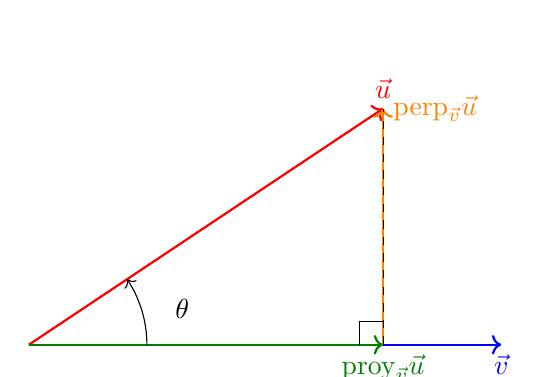
\begin{tikzpicture}[scale=1.5]
  % Vector base
  \draw[->, thick, blue] (0,0) -- (4,0) node[below] {$\vec{v}$};
  
  % Vector a proyectar
  \draw[->, thick, red] (0,0) -- (3,2) node[above] {$\vec{u}$};
  
  % Proyección
  \draw[->, thick, green!50!black] (0,0) -- (3,0) node[below] {$\text{proy}_{\vec{v}}\vec{u}$};
  
  % Componente perpendicular
  \draw[->, thick, orange] (3,0) -- (3,2) node[right] {$\text{perp}_{\vec{v}}\vec{u}$};
  
  % Línea perpendicular
  \draw[dashed] (3,0) -- (3,2);
  
  % Ángulo recto
  \draw (2.8,0) -- (2.8,0.2) -- (3,0.2);
  
  % Ángulo theta
  \draw[->] (1,0) arc (0:33.69:1);
  \node at (1.3,0.3) {$\theta$};
\end{tikzpicture}
\end{center}

\subsection{Trabajo Mecánico}

El trabajo realizado por una fuerza $\vec{F}$ sobre un desplazamiento $\vec{d}$:

\[
\boxed{
W = \vec{F} \cdot \vec{d} = |\vec{F}||\vec{d}|\cos\theta
}
\]

\section{Producto Cruz (Vectorial)}

\subsection{Definición (solo en 3D)}

\[
\boxed{
\vec{u} \times \vec{v} = \begin{vmatrix}
\vec{i} & \vec{j} & \vec{k} \\
u_1 & u_2 & u_3 \\
v_1 & v_2 & v_3
\end{vmatrix}
}
\]

\[
\boxed{
\vec{u} \times \vec{v} = (u_2v_3 - u_3v_2)\vec{i} - (u_1v_3 - u_3v_1)\vec{j} + (u_1v_2 - u_2v_1)\vec{k}
}
\]

\subsection{Propiedades del Producto Cruz}

\begin{enumerate}
  \item \textbf{Anticonmutativa}: $\vec{u} \times \vec{v} = -(\vec{v} \times \vec{u})$
  
  \item \textbf{Distributiva}: $\vec{u} \times (\vec{v} + \vec{w}) = \vec{u} \times \vec{v} + \vec{u} \times \vec{w}$
  
  \item \textbf{Asociativa con escalares}: $(k\vec{u}) \times \vec{v} = k(\vec{u} \times \vec{v}) = \vec{u} \times (k\vec{v})$
  
  \item \textbf{Producto consigo mismo}: $\vec{v} \times \vec{v} = \vec{0}$
  
  \item \textbf{Con el vector cero}: $\vec{v} \times \vec{0} = \vec{0}$
  
  \item \textbf{Vectores paralelos}: $\vec{u} \parallel \vec{v} \Leftrightarrow \vec{u} \times \vec{v} = \vec{0}$
\end{enumerate}

\subsection{Magnitud del Producto Cruz}

\[
\boxed{
|\vec{u} \times \vec{v}| = |\vec{u}||\vec{v}|\sin\theta
}
\]

donde $\theta$ es el ángulo entre los vectores.

\subsection{Dirección del Producto Cruz}

El vector $\vec{u} \times \vec{v}$ es perpendicular tanto a $\vec{u}$ como a $\vec{v}$, y su dirección sigue la \textbf{regla de la mano derecha}.

\[
\boxed{
(\vec{u} \times \vec{v}) \perp \vec{u} \quad \text{y} \quad (\vec{u} \times \vec{v}) \perp \vec{v}
}
\]

\subsection{Productos Cruz de Vectores Unitarios}

\[
\boxed{
\begin{aligned}
\vec{i} \times \vec{j} &= \vec{k} \quad , \quad \vec{j} \times \vec{i} = -\vec{k} \\[6pt]
\vec{j} \times \vec{k} &= \vec{i} \quad , \quad \vec{k} \times \vec{j} = -\vec{i} \\[6pt]
\vec{k} \times \vec{i} &= \vec{j} \quad , \quad \vec{i} \times \vec{k} = -\vec{j}
\end{aligned}
}
\]

\subsection{Aplicaciones del Producto Cruz}

\subsubsection{Área de paralelogramo}

El área del paralelogramo formado por $\vec{u}$ y $\vec{v}$:

\[
\boxed{
A_{\text{paralelogramo}} = |\vec{u} \times \vec{v}|
}
\]

\subsubsection{Área de triángulo}

El área del triángulo formado por $\vec{u}$ y $\vec{v}$:

\[
\boxed{
A_{\text{triángulo}} = \frac{1}{2}|\vec{u} \times \vec{v}|
}
\]

\subsubsection{Momento de torsión (torque)}

\[
\boxed{
\vec{\tau} = \vec{r} \times \vec{F}
}
\]

donde $\vec{r}$ es el vector posición y $\vec{F}$ es la fuerza.

\subsubsection{Velocidad angular}

\[
\boxed{
\vec{v} = \vec{\omega} \times \vec{r}
}
\]

donde $\vec{\omega}$ es la velocidad angular.

\subsection{Producto Cruz en 2D (Determinante)}

En 2D, el producto cruz se reduce a un escalar:

\[
\boxed{
\vec{u} \times \vec{v} = u_xv_y - u_yv_x
}
\]

\textbf{Interpretación geométrica}:
\begin{itemize}
  \item Si es positivo: $\vec{v}$ está a la izquierda de $\vec{u}$ (giro antihorario)
  \item Si es negativo: $\vec{v}$ está a la derecha de $\vec{u}$ (giro horario)
  \item Si es cero: $\vec{u}$ y $\vec{v}$ son colineales
\end{itemize}

\section{Producto Triple}

\subsection{Producto Triple Escalar}

\[
\boxed{
\vec{u} \cdot (\vec{v} \times \vec{w}) = \begin{vmatrix}
u_1 & u_2 & u_3 \\
v_1 & v_2 & v_3 \\
w_1 & w_2 & w_3
\end{vmatrix}
}
\]

\textbf{Propiedades}:
\begin{itemize}
  \item Invariante bajo permutaciones cíclicas: $\vec{u} \cdot (\vec{v} \times \vec{w}) = \vec{v} \cdot (\vec{w} \times \vec{u}) = \vec{w} \cdot (\vec{u} \times \vec{v})$
  \item Cambia de signo con permutación no cíclica: $\vec{u} \cdot (\vec{w} \times \vec{v}) = -\vec{u} \cdot (\vec{v} \times \vec{w})$
\end{itemize}

\subsubsection{Volumen de paralelepípedo}

\[
\boxed{
V_{\text{paralelepípedo}} = |\vec{u} \cdot (\vec{v} \times \vec{w})|
}
\]

\subsubsection{Volumen de tetraedro}

\[
\boxed{
V_{\text{tetraedro}} = \frac{1}{6}|\vec{u} \cdot (\vec{v} \times \vec{w})|
}
\]

\subsubsection{Coplanaridad}

Tres vectores son coplanares si y solo si:

\[
\boxed{
\vec{u} \cdot (\vec{v} \times \vec{w}) = 0
}
\]

\subsection{Producto Triple Vectorial}

\[
\boxed{
\vec{u} \times (\vec{v} \times \vec{w}) = (\vec{u} \cdot \vec{w})\vec{v} - (\vec{u} \cdot \vec{v})\vec{w}
}
\]

\textbf{Identidad BAC-CAB}:

\[
\boxed{
\vec{u} \times (\vec{v} \times \vec{w}) = \vec{v}(\vec{u} \cdot \vec{w}) - \vec{w}(\vec{u} \cdot \vec{v})
}
\]

\textbf{Nota}: $(\vec{u} \times \vec{v}) \times \vec{w} \neq \vec{u} \times (\vec{v} \times \vec{w})$ (no es asociativo)

\subsection{Identidad de Jacobi}

\[
\boxed{
\vec{u} \times (\vec{v} \times \vec{w}) + \vec{v} \times (\vec{w} \times \vec{u}) + \vec{w} \times (\vec{u} \times \vec{v}) = \vec{0}
}
\]

\subsection{Identidad de Lagrange}

\[
\boxed{
(\vec{u} \times \vec{v}) \cdot (\vec{w} \times \vec{z}) = (\vec{u} \cdot \vec{w})(\vec{v} \cdot \vec{z}) - (\vec{u} \cdot \vec{z})(\vec{v} \cdot \vec{w})
}
\]

Caso especial ($\vec{w} = \vec{u}$, $\vec{z} = \vec{v}$):

\[
\boxed{
|\vec{u} \times \vec{v}|^2 = |\vec{u}|^2|\vec{v}|^2 - (\vec{u} \cdot \vec{v})^2
}
\]

\section{Rectas en el Espacio}

\subsection{Ecuación Vectorial de la Recta}

Una recta que pasa por el punto $P_0$ con vector dirección $\vec{v}$:

\[
\boxed{
\vec{r}(t) = \vec{r_0} + t\vec{v}
}
\]

o en componentes:

\[
\boxed{
\vec{r}(t) = (x_0, y_0, z_0) + t(a, b, c)
}
\]

\subsection{Ecuación Paramétrica de la Recta}

\[
\boxed{
\begin{cases}
x = x_0 + at \\
y = y_0 + bt \\
z = z_0 + ct
\end{cases}
}
\]

donde $(a, b, c)$ es el vector dirección y $t \in \mathbb{R}$ es el parámetro.

\subsection{Ecuación Simétrica de la Recta}

Si $a, b, c \neq 0$:

\[
\boxed{
\frac{x - x_0}{a} = \frac{y - y_0}{b} = \frac{z - z_0}{c}
}
\]

\subsection{Ecuación de la Recta por Dos Puntos}

Recta que pasa por $P_1(x_1, y_1, z_1)$ y $P_2(x_2, y_2, z_2)$:

\[
\boxed{
\vec{r}(t) = (1-t)P_1 + tP_2 = P_1 + t(P_2 - P_1)
}
\]

Vector dirección: $\vec{v} = P_2 - P_1$

\subsection{Punto en una Recta}

Un punto $P$ está en la recta si existe un valor de $t$ tal que:

\[
P = P_0 + t\vec{v}
\]

\subsection{Rectas en 2D}

\subsubsection{Forma punto-pendiente}

\[
\boxed{
y - y_0 = m(x - x_0)
}
\]

\subsubsection{Forma general}

\[
\boxed{
Ax + By + C = 0
}
\]

Vector dirección: $\vec{v} = (-B, A)$ o $(B, -A)$

Vector normal: $\vec{n} = (A, B)$

\subsubsection{Forma vectorial en 2D}

\[
\boxed{
\vec{r}(t) = (x_0, y_0) + t(a, b)
}
\]

\subsection{Distancia de un Punto a una Recta}

\subsubsection{En 3D (usando producto cruz)}

Distancia del punto $P$ a la recta que pasa por $P_0$ con dirección $\vec{v}$:

\[
\boxed{
d = \frac{|\overrightarrow{P_0P} \times \vec{v}|}{|\vec{v}|}
}
\]

\subsubsection{En 2D (usando forma general)}

Distancia del punto $(x_0, y_0)$ a la recta $Ax + By + C = 0$:

\[
\boxed{
d = \frac{|Ax_0 + By_0 + C|}{\sqrt{A^2 + B^2}}
}
\]

\subsection{Distancia entre Dos Rectas}

\subsubsection{Rectas paralelas}

Si $\vec{v_1} \parallel \vec{v_2}$ (misma dirección):

\[
\boxed{
d = \frac{|\overrightarrow{P_1P_2} \times \vec{v_1}|}{|\vec{v_1}|}
}
\]

\subsubsection{Rectas que se cruzan (skew lines)}

\[
\boxed{
d = \frac{|\overrightarrow{P_1P_2} \cdot (\vec{v_1} \times \vec{v_2})|}{|\vec{v_1} \times \vec{v_2}|}
}
\]

\subsection{Ángulo entre Dos Rectas}

\[
\boxed{
\cos\theta = \frac{|\vec{v_1} \cdot \vec{v_2}|}{|\vec{v_1}||\vec{v_2}|}
}
\]

\subsection{Condiciones Especiales}

\subsubsection{Rectas paralelas}

\[
\boxed{
\vec{v_1} \parallel \vec{v_2} \Leftrightarrow \vec{v_1} = k\vec{v_2}
}
\]

\subsubsection{Rectas perpendiculares}

\[
\boxed{
\vec{v_1} \perp \vec{v_2} \Leftrightarrow \vec{v_1} \cdot \vec{v_2} = 0
}
\]

\subsubsection{Rectas coplanares}

Dos rectas son coplanares si:

\[
\boxed{
\overrightarrow{P_1P_2} \cdot (\vec{v_1} \times \vec{v_2}) = 0
}
\]

\section{Planos en el Espacio}

\subsection{Ecuación Vectorial del Plano}

Un plano que pasa por el punto $P_0$ con vectores directores $\vec{u}$ y $\vec{v}$:

\[
\boxed{
\vec{r}(s, t) = \vec{r_0} + s\vec{u} + t\vec{v}
}
\]

\subsection{Ecuación Normal del Plano}

Un plano con vector normal $\vec{n} = (A, B, C)$ que pasa por $P_0(x_0, y_0, z_0)$:

\[
\boxed{
\vec{n} \cdot (\vec{r} - \vec{r_0}) = 0
}
\]

o:

\[
\boxed{
A(x - x_0) + B(y - y_0) + C(z - z_0) = 0
}
\]

\subsection{Ecuación General del Plano}

\[
\boxed{
Ax + By + Cz + D = 0
}
\]

donde $\vec{n} = (A, B, C)$ es el vector normal al plano.

\subsection{Vector Normal al Plano}

Si el plano está definido por dos vectores $\vec{u}$ y $\vec{v}$:

\[
\boxed{
\vec{n} = \vec{u} \times \vec{v}
}
\]

\subsection{Plano por Tres Puntos}

Dado tres puntos $P_1, P_2, P_3$, el vector normal es:

\[
\boxed{
\vec{n} = \overrightarrow{P_1P_2} \times \overrightarrow{P_1P_3}
}
\]

\subsection{Intersección de Planos}

\subsubsection{Planos paralelos}

\[
\boxed{
\vec{n_1} \parallel \vec{n_2} \Leftrightarrow \vec{n_1} = k\vec{n_2}
}
\]

\subsubsection{Planos perpendiculares}

\[
\boxed{
\vec{n_1} \perp \vec{n_2} \Leftrightarrow \vec{n_1} \cdot \vec{n_2} = 0
}
\]

\subsubsection{Línea de intersección}

Si dos planos se intersectan, forman una recta con vector dirección:

\[
\boxed{
\vec{v} = \vec{n_1} \times \vec{n_2}
}
\]

\subsection{Ángulo entre Dos Planos}

\[
\boxed{
\cos\theta = \frac{|\vec{n_1} \cdot \vec{n_2}|}{|\vec{n_1}||\vec{n_2}|}
}
\]

\subsection{Distancia de un Punto a un Plano}

Distancia del punto $P(x_0, y_0, z_0)$ al plano $Ax + By + Cz + D = 0$:

\[
\boxed{
d = \frac{|Ax_0 + By_0 + Cz_0 + D|}{\sqrt{A^2 + B^2 + C^2}}
}
\]

\subsection{Distancia entre Dos Planos Paralelos}

Para planos $Ax + By + Cz + D_1 = 0$ y $Ax + By + Cz + D_2 = 0$:

\[
\boxed{
d = \frac{|D_2 - D_1|}{\sqrt{A^2 + B^2 + C^2}}
}
\]

\subsection{Proyección de un Punto sobre un Plano}

La proyección del punto $P$ sobre el plano con normal $\vec{n}$ que pasa por $P_0$:

\[
\boxed{
P' = P - \frac{\vec{n} \cdot \overrightarrow{P_0P}}{|\vec{n}|^2}\vec{n}
}
\]

\subsection{Reflexión de un Punto sobre un Plano}

\[
\boxed{
P'' = P - 2\frac{\vec{n} \cdot \overrightarrow{P_0P}}{|\vec{n}|^2}\vec{n}
}
\]

\subsection{Intersección de Recta y Plano}

Recta: $\vec{r}(t) = \vec{r_0} + t\vec{v}$

Plano: $\vec{n} \cdot (\vec{r} - \vec{p}) = 0$

Punto de intersección en:

\[
\boxed{
t = \frac{\vec{n} \cdot (\vec{p} - \vec{r_0})}{\vec{n} \cdot \vec{v}}
}
\]

\textbf{Casos especiales}:
\begin{itemize}
  \item Si $\vec{n} \cdot \vec{v} = 0$ y $\vec{n} \cdot (\vec{p} - \vec{r_0}) = 0$: la recta está contenida en el plano
  \item Si $\vec{n} \cdot \vec{v} = 0$ y $\vec{n} \cdot (\vec{p} - \vec{r_0}) \neq 0$: la recta es paralela al plano
\end{itemize}

\section{Sistemas de Coordenadas}

\subsection{Coordenadas Cartesianas (Rectangulares)}

\[
\boxed{
P = (x, y, z)
}
\]

\subsection{Coordenadas Cilíndricas}

\[
\boxed{
P = (r, \theta, z)
}
\]

\textbf{Conversión a cartesianas}:

\[
\boxed{
\begin{cases}
x = r\cos\theta \\
y = r\sin\theta \\
z = z
\end{cases}
}
\]

\textbf{Conversión de cartesianas}:

\[
\boxed{
\begin{cases}
r = \sqrt{x^2 + y^2} \\
\theta = \arctan(y/x) \\
z = z
\end{cases}
}
\]

\subsection{Coordenadas Esféricas}

\[
\boxed{
P = (\rho, \theta, \phi)
}
\]

donde:
\begin{itemize}
  \item $\rho$: distancia desde el origen
  \item $\theta$: ángulo azimutal (en el plano $xy$)
  \item $\phi$: ángulo polar (desde el eje $z$)
\end{itemize}

\textbf{Conversión a cartesianas}:

\[
\boxed{
\begin{cases}
x = \rho\sin\phi\cos\theta \\
y = \rho\sin\phi\sin\theta \\
z = \rho\cos\phi
\end{cases}
}
\]

\textbf{Conversión de cartesianas}:

\[
\boxed{
\begin{cases}
\rho = \sqrt{x^2 + y^2 + z^2} \\
\theta = \arctan(y/x) \\
\phi = \arccos(z/\rho)
\end{cases}
}
\]

\subsection{Elementos de Volumen}

\textbf{Cartesianas}: $dV = dx\,dy\,dz$

\textbf{Cilíndricas}: $dV = r\,dr\,d\theta\,dz$

\textbf{Esféricas}: $dV = \rho^2\sin\phi\,d\rho\,d\theta\,d\phi$

\section{Bases Vectoriales}

\subsection{Base Ortonormal}

Una base $\{\vec{e_1}, \vec{e_2}, \vec{e_3}\}$ es ortonormal si:

\[
\boxed{
\vec{e_i} \cdot \vec{e_j} = \delta_{ij} = \begin{cases}
1 & \text{si } i = j \\
0 & \text{si } i \neq j
\end{cases}
}
\]

\subsection{Cambio de Base}

Si $\vec{v} = v_1\vec{e_1} + v_2\vec{e_2} + v_3\vec{e_3}$ en una base ortonormal:

\[
\boxed{
v_i = \vec{v} \cdot \vec{e_i}
}
\]

\subsection{Matriz de Rotación}

Para rotar un vector alrededor del origen:

\textbf{Rotación en 2D por ángulo $\theta$}:

\[
\boxed{
R(\theta) = \begin{pmatrix}
\cos\theta & -\sin\theta \\
\sin\theta & \cos\theta
\end{pmatrix}
}
\]

\textbf{Rotación en 3D alrededor del eje $z$}:

\[
\boxed{
R_z(\theta) = \begin{pmatrix}
\cos\theta & -\sin\theta & 0 \\
\sin\theta & \cos\theta & 0 \\
0 & 0 & 1
\end{pmatrix}
}
\]

\subsection{Proceso de Gram-Schmidt}

Para ortogonalizar un conjunto de vectores $\{\vec{v_1}, \vec{v_2}, \vec{v_3}\}$:

\[
\boxed{
\begin{aligned}
\vec{u_1} &= \vec{v_1} \\[6pt]
\vec{u_2} &= \vec{v_2} - \text{proy}_{\vec{u_1}}\vec{v_2} \\[6pt]
\vec{u_3} &= \vec{v_3} - \text{proy}_{\vec{u_1}}\vec{v_3} - \text{proy}_{\vec{u_2}}\vec{v_3}
\end{aligned}
}
\]

Luego normalizar: $\vec{e_i} = \frac{\vec{u_i}}{|\vec{u_i}|}$

\section{Operaciones Avanzadas}

\subsection{Gradiente (campo escalar a vectorial)}

\[
\boxed{
\nabla f = \frac{\partial f}{\partial x}\vec{i} + \frac{\partial f}{\partial y}\vec{j} + \frac{\partial f}{\partial z}\vec{k}
}
\]

\subsection{Divergencia (campo vectorial a escalar)}

\[
\boxed{
\nabla \cdot \vec{F} = \frac{\partial F_x}{\partial x} + \frac{\partial F_y}{\partial y} + \frac{\partial F_z}{\partial z}
}
\]

\subsection{Rotacional (campo vectorial a vectorial)}

\[
\boxed{
\nabla \times \vec{F} = \begin{vmatrix}
\vec{i} & \vec{j} & \vec{k} \\
\frac{\partial}{\partial x} & \frac{\partial}{\partial y} & \frac{\partial}{\partial z} \\
F_x & F_y & F_z
\end{vmatrix}
}
\]

\subsection{Laplaciano}

\[
\boxed{
\nabla^2 f = \nabla \cdot \nabla f = \frac{\partial^2 f}{\partial x^2} + \frac{\partial^2 f}{\partial y^2} + \frac{\partial^2 f}{\partial z^2}
}
\]

\subsection{Identidades Vectoriales Importantes}

\[
\boxed{
\begin{aligned}
\nabla \times (\nabla f) &= \vec{0} \\[6pt]
\nabla \cdot (\nabla \times \vec{F}) &= 0 \\[6pt]
\nabla \times (\nabla \times \vec{F}) &= \nabla(\nabla \cdot \vec{F}) - \nabla^2\vec{F} \\[6pt]
\nabla(fg) &= f\nabla g + g\nabla f \\[6pt]
\nabla \cdot (f\vec{F}) &= f(\nabla \cdot \vec{F}) + \vec{F} \cdot \nabla f \\[6pt]
\nabla \times (f\vec{F}) &= f(\nabla \times \vec{F}) + (\nabla f) \times \vec{F}
\end{aligned}
}
\]

\end{document}
